\documentclass[a4paper, 11pt]{article}
%twocolumn
%\usepackage[a4paper, top=25mm, bottom=25mm, left=15mm, right=12mm]{geometry}
%\setlength{\columnsep}{5mm} % Adjust column separation if needed
\usepackage[a4paper, margin=0.8in]{geometry}
%\setlength{\columnwidth}{88mm}
\usepackage[utf8]{inputenc}
\usepackage[T1]{fontenc}
\usepackage[english]{babel} 

\newcommand{\quotes}[1]{``#1''}

% Graphics and Floats
\usepackage{graphicx}
\usepackage{float}
\usepackage{incgraph}
\usepackage{tikz}
\usepackage{pgfplotstable} 
\usepackage{pgfplots}
\pgfplotsset{compat=1.18}
\usepackage{wrapfig}
\usepackage{subcaption}

% Math and Symbols
\usepackage{amsmath}
\usepackage{amssymb}
\usepackage{amsthm}
%\usepackage{showframe}
% Typography
\usepackage{widows-and-orphans}
\usepackage{xspace}
\usepackage[indent]{parskip}
\usepackage{indentfirst}
\usepackage[final,nopatch=footnote]{microtype}
\usepackage[all]{nowidow}

\usepackage{xcolor}
\definecolor{backcolour}{rgb}{0.95,0.95,0.92}
\xdefinecolor{gray}{rgb}{0.4,0.4,0.4}
\xdefinecolor{blue}{RGB}{58,95,205}% R's royalblue3; #3A5FCD

% Code Listings
\usepackage{listings}[captionpos=b]
\usepackage{fancyvrb}
\usepackage{bm}
\usepackage{textcomp}
\usepackage[ruled,vlined]{algorithm2e}
\usepackage{hyperref}
% Bibliography
\usepackage[style=ieee, sorting=none]{biblatex}
\addbibresource{references.bib}

\usepackage{csquotes}


\title{Randomized Algorithms (RA-MIRI): \\
        Assignment \#1
        }
\author{%   
    Marc Díaz (marc.diaz.calderon@estudiantat.upc.edu) 
}
\date{October 2024}

\begin{document}

\maketitle

\section{Code Solution}

As explained in the assignment, the Galton board is a probabilistic model where balls drop through a series of pegs and end up in bins at the bottom. Each bin represents a possible outcome based on the random path taken by the ball.

We will assume that only well constructed boards are possible, hence $\forall N \in \mathbb{N}^+$ number of bins, there are exactly $N-1$ rows of pegs. For the solution proposed, we do not need to keep track of the whole matrix, just the current position of the ball. The pseudocode for simulating the ball's trajectory is given in Algorithm \ref{algo:ballSimulation}. The algorithm initializes the ball at the top (height 0) and simulates its movement down the board until the $N-1$ peg row.

\begin{algorithm}[h]
    \caption{Ball Simulation Algorithm  - $\mathcal{O}(N)$}
    \label{algo:ballSimulation}
    \SetAlgoLined  
    \SetKwFunction{SimulateBall}{SimulateBall}
    \SetKwInOut{Input}{Input}
    \SetKwInOut{Output}{Output}

    \Input{$N$ -- number of bins ($N \in \mathbb{N}^+$)}
    \Output{Updated bin counts in array $\mathit{bins\_}$}

    \BlankLine
    
    \SetKwData{CurrentHeight}{current\_height}
    \SetKwData{Position}{position}
    \SetKwData{Rand}{random\_value}
    \SetKwData{Bins}{bins\_}

    \CurrentHeight $\gets 0$\;
    \Position $\gets N - 1$ \tcp*{Start position}
    
    \While{\CurrentHeight $<$ $N - 1$}{
        \Rand $\gets$ a random number between 0 and 1\;
        \eIf{\Rand $<$ 0.5}{
            Increment \Position by 1\;
        }{
            Decrement \Position by 1\;
        }
        Increment \CurrentHeight by 1\;
    }

    \tcp{Update the bin corresponding to the final position}
    Increment $\Bins\left[\Position / 2\right]$\;

\end{algorithm}

The code solution has been implemented in C++ and can be found in \href{https://github.com/MDCmarc/RA-Assigment1}{this GitHub repo} - (https://github.com/MDCmarc/RA-Assigment1). 
For random number generation, we utilized the \texttt{mt19937} random engine, which is based on the classic Mersenne Twister algorithm~\cite{MersenneTwister}. 

For the experimentation, since the outcome of each ball is independent of the others, we simulated $K$ balls, where $K \in \mathbb{N}^+$, using parallelization through OpenMP.

At the end of the simulation, the position is guaranteed to be both positive and even.

\subsection{Correctness}
\subsubsection*{Even Position}
As we saw, we initialize \texttt{position} as $N-1$. Then we have two cases:
\begin{itemize}
    \item \textbf{Case 1: Even Number of Bins.} If $N$ is even, the initial position is odd. With each step, the ball either increments or decrements its position, thus changing its parity (odd to even or even to odd). Since there are exactly $N-1$ peg rows, the ball makes an odd number of moves, ensuring that the final position is even.

    \item \textbf{Case 2: Odd Number of Bins.} If $N$ is odd, the initial position is even. The ball makes then $N-1$ (an even number) moves, preserving the initial parity, so the final position remains even.
\end{itemize}

\subsubsection*{Positive Position}
The ball starts at $N-1$, the end of the array of bins. After $N-1$ iterations, the minimum possible position is 0 (if all moves were -1), while the maximum possible position is $2 \cdot (N-1)$ (if all moves were +1). This ensures that the ball's final position is always non-negative.

Finally, incrementing exactly the bin at $\text{position}/2$ will map correctly each position to its corresponding bin. 


\section{Experimentation}

In our experiments, we ran the algorithm with varying parameters, specifically altering the number of bins and the number of balls. All simulations are stored in the \texttt{Simulations} folder within the project.

Initially, we aimed to compare the simulation results with the theoretical Binomial distribution that models them. To facilitate this comparison, we transformed the simulation output from showing the number of balls per bin to presenting the proportion of balls allocated to each bin. This transformation allowed us to obtain empirical probabilities.

These empirical probabilities were then compared against the theoretical probabilities derived from the Binomial distribution with identical parameters. Figure~\ref{fig:comparison} shows three different comparisons. In Subfigure~\subref{subfig:7bins} we present the empirical probabilities obtained from executing the Galton board simulation with 10,000 balls and 7 bins (resulting in 6 choices). For clarity, the theoretical values have been slightly shifted to the right in all plots. The results indicate a strong similarity between the empirical and theoretical probabilities. With the error bars calculated using the formula $\sqrt{N \cdot p_{i,n}\cdot q_{i,n}}$ the theoretical values mostly fall within the expected error bounds, with very few instances where they slightly exceed these bounds.

Subfigure~\subref{subfig:21bins} and Subfigure~\subref{subfig:41bins} follow a similar approach, but with 21 and 41 bins, respectively. In these cases, the empirical and theoretical values also coincide in the majority of cases within their respective error bars. It is important to note that all three scenarios utilized a substantial number of balls; the following experiments will explore how varying the number of balls influences the outcomes.

\begin{figure}[H]
    \centering
    % First plot
    \begin{subfigure}[t]{0.45\textwidth}
        \centering
        \begin{tikzpicture}[
            declare function={
                binom(\k,\n,\p)=\n!/(\k!*(\n-\k)!)*\p^\k*(1-\p)^(\n-\k);
                stddev(\N,\p)=sqrt(\N * \p * (1-\p));
        }]
            \pgfplotstableread[col sep=comma]{Simulations/simulation_7_10000.csv}\datatable
            \pgfmathsetmacro{\totalballs}{10000}
            \begin{axis}[
                samples at={0,...,6},
                yticklabel style={
                    /pgf/number format/fixed,
                    /pgf/number format/fixed zerofill,
                    /pgf/number format/precision=2
                },
                ybar=0pt, 
                bar width=1,
                xlabel={$K$},
                ylabel={$P[X=k]$},
                ymin=0,
                legend style={at={(1.35,1.1)}, anchor=north east}
            ]
                % Binomial distribution
                \addplot[
                    y filter/.expression={\thisrow{balls} / \totalballs},
                    fill=blue,
                    bar width=0.3cm,
                    opacity=0.6,
                ] table[x=bin, y=balls] {\datatable};\addlegendentry{Empirical}
                
                % Theoretical binomial distribution
                \addplot [fill=orange, fill opacity=0.5] {binom(x,6,0.5)};\addlegendentry{Theoretical}

                % Plot the error bars
                 \addplot[
                    black, mark options={black, scale=0.75},
                    smooth,
                    error bars/.cd,
                        y dir=both, 
                        y explicit,
                        error bar style={line width=1pt, color=red},
                ] table[
                    x=bin, 
                    y expr={\thisrow{balls} / \totalballs}, 
                    y error expr={stddev(\totalballs, binom(\thisrow{bin}, 6, 0.5)) / \totalballs}
                ] {\datatable};\addlegendentry{Standard Deviation}
            \end{axis}
        \end{tikzpicture}
        \caption{Distribution of balls across 7 bins with empirical and theoretical probabilities.}
        \label{subfig:7bins}
    \end{subfigure}
    \hfill
    \begin{subfigure}[t]{0.45\textwidth}
        \centering
        \begin{tikzpicture}[
            declare function={binom(\k,\n,\p)=\n!/(\k!*(\n-\k)!)*\p^\k*(1-\p)^(\n-\k);
            stddev(\N,\p)=sqrt(\N * \p * (1-\p));
        }]
            \pgfplotstableread[col sep=comma]{Simulations/simulation_21_10000.csv}\datatable
            \pgfmathsetmacro{\totalballs}{10000}
            \begin{axis}[
                samples at={0,...,20},
                yticklabel style={
                    /pgf/number format/fixed,
                    /pgf/number format/fixed zerofill,
                    /pgf/number format/precision=2
                },
                ybar=0pt, 
                bar width=1,
                xlabel={$K$},
                ylabel={$P[X=k]$},
                ymin=0,
                ylabel near ticks, yticklabel pos=right
            ]
                % Binomial distribution
                \addplot+[
                    y filter/.expression={\thisrow{balls} / \totalballs},
                    fill=blue,
                    bar width=0.3cm,
                    opacity=0.6,
                ] table[x=bin, y=balls] {\datatable};
                
                % Theoretical binomial distribution
                \addplot [fill=orange, fill opacity=0.5] {binom(x,20,0.5)};
                
                % Plot the error bars
                \addplot[
                    black,
                    smooth,
                    error bars/.cd,
                        y dir=both, 
                        y explicit,
                        error bar style={line width=1pt, color=red},
                ] table[
                    x=bin, 
                    y expr={\thisrow{balls} / \totalballs}, 
                    y error expr={stddev(\totalballs, binom(\thisrow{bin}, 20, 0.5)) / \totalballs}
                ] {\datatable};
            \end{axis}
        \end{tikzpicture}
        \caption{Distribution of balls across 21 bins with empirical and theoretical probabilities.}
        \label{subfig:21bins}
    \end{subfigure}
    \vskip\baselineskip
    % third plot
    \begin{subfigure}[t]{0.45\textwidth}
        \centering
        \begin{tikzpicture}[
            declare function={
                binom(\k,\n,\p)=\n!/(\k!*(\n-\k)!)*\p^\k*(1-\p)^(\n-\k);
                stddev(\N,\p)=sqrt(\N * \p * (1-\p));
                }]
            \pgfplotstableread[col sep=comma]{Simulations/simulation_41_10000.csv}\datatable
            \pgfmathsetmacro{\totalballs}{10000}
            \begin{axis}[
                samples at={0,...,40},
                yticklabel style={
                    /pgf/number format/fixed,
                    /pgf/number format/fixed zerofill,
                    /pgf/number format/precision=2
                },
                ybar=0pt, bar width=1,
                xlabel={$K$},
                ylabel={$P[X=k]$},
                ymin=0,
                legend style={at={(1.25,1)}, anchor=north east}
            ]
                % Binomial distribution
                \addplot+[
                    y filter/.expression={\thisrow{balls} / \totalballs},
                    fill=blue,
                    bar width=0.1cm,
                    opacity=0.6,
                ] table[x=bin, y=balls] {\datatable};\addlegendentry{Empirical}
                
                % Theoretical binomial distribution
                \addplot [fill=orange, fill opacity=0.5] {binom(x,40,0.5)};\addlegendentry{Theoretical}
                % Plot the error bars
                \addplot[
                    black,
                    smooth,
                    error bars/.cd,
                        y dir=both, 
                        y explicit,
                        error bar style={line width=1pt, color=red},
                ] table[
                    x=bin, 
                    y expr={\thisrow{balls} / \totalballs}, 
                    y error expr={stddev(\totalballs, binom(\thisrow{bin}, 40, 0.5)) / \totalballs}
                ] {\datatable};\addlegendentry{Standard Deviation}
            \end{axis}
        \end{tikzpicture}
        \caption{Distribution of balls across 41 bins with empirical and theoretical probabilities.}
        \label{subfig:41bins}
    \end{subfigure}
    
    \caption{Comparison of empirical and theoretical probabilities across different bin distributions. Each subplot illustrates the distribution of balls in the bins alongside their theoretical counterparts and error bars indicating the standard deviation.}
    \label{fig:comparison}
\end{figure}

In this second part of our analysis, we investigate the agreement between the empirical binomial distribution and its corresponding normal approximation. We assume that the distribution obtained from our experiments follows the previously established binomial distribution  $Bin(n,1/2)$.

Figure~\ref{fig:normals} shows 2 comparisons between the empirical Binomial from the experiments, and the theoretical normal distribution associated $\mathcal{N}(n/2,n/4)$ using a sample size of 10,000 trials. Subfigure~\ref{subfig:normal7} shows the comparison with only 7 bins, hence the difference is quite notorious, however, in Subfigure~\ref{subfig:normal71} where we are using now more bins (71 bins) the empirical Binomial is much more close to the normal distribution. However, visual comparisons alone are insufficient for a comprehensive analysis. 
Therefore, we created Figure~\ref{fig:error_analysis}, which shows the mean square error between the probability density function of the normal distribution and the empirical results from our experiments. This analysis is conducted for eight different sample sizes, with the number of bins varying in the form $5*i +1$. The result show what already was hinted by the naive comparison, more number of bins implies more similarity. However, we were ignoring the possibility of changing the ball number. It comes clear now the impact of sample size on the error; having a larger number of balls significantly reduces the mean square error, hence giving more accurate approximations.


\begin{figure}[!ht] 
    \captionsetup[subfigure]{justification=centering,labelformat=brace}
    \centering
    \subcaptionbox{{\label{subfig:normal7}}Comparison of the binomial distribution with \\ 7 bins (6 decisions) and its normal approximation.}[.5\textwidth]{%
    \begin{tikzpicture}
        \pgfplotstableread[col sep=comma]{Simulations/simulation_7_10000.csv}\datatable
        \pgfmathsetmacro{\totalballs}{10000}
        \pgfplotstablegetrowsof{\datatable}
        \pgfmathsetmacro{\nbins}{\pgfplotsretval - 1}
        \pgfmathsetmacro{\muK}{\nbins / 2.0}
        \pgfmathsetmacro{\variance}{\nbins / 4.0}
        \begin{axis}[
            ybar,
            xlabel={$K$},
            ylabel={$P[X=k]$},
            enlarge x limits=0.1,
            title={},
            ymin=0,
            xtick={0,1,2,3,4,5,6},
            grid=major,
            legend style={at={(0.5,-0.2)}, anchor=north, legend columns=1},
        ] % Binomial distribution
            \addplot+[
                y filter/.expression={\thisrow{balls} / \totalballs},
                bar width=0.9cm,
                fill=blue,
                opacity=0.6,
            ] table[x=bin, y=balls] {\datatable};
            \addlegendentry{Binomial $Bin(\nbins, 0.5)$}
            % Normal distribution as a thin line
            \addplot+[
                domain=0:\nbins, 
                samples=100, 
                smooth,
                thick,
                only marks,
                color=black,
            ]{1/(sqrt(2*pi*\variance)) * exp(-((x-\muK)^2)/(2*\variance))};
            \addlegendentry{Normal $\mathcal{N}(\mu=\muK,\sigma^2=\variance)$}
        \end{axis}
    \end{tikzpicture}}%%
    \subcaptionbox{{\label{subfig:normal71}}Comparison of the binomial distribution with 71 bins \\ (70 decisions) and its normal approximation.}[.5\textwidth]{%
    \begin{tikzpicture}
        \pgfplotstableread[col sep=comma]{Simulations/simulation_71_10000.csv}\datatable
        \pgfmathsetmacro{\totalballs}{10000}
        \pgfplotstablegetrowsof{\datatable}
        \pgfmathsetmacro{\nbins}{\pgfplotsretval - 1}
        \pgfmathsetmacro{\muK}{\nbins / 2.0}
        \pgfmathsetmacro{\variance}{\nbins / 4.0}
        \begin{axis}[
            ybar,
            xlabel={$K$},
            ylabel near ticks, yticklabel pos=right,
            ylabel={$P[X=k]$},
            enlarge x limits=0,
            title={},
            ymin=0,
            grid=major,
            %xtick={0,2,4,6,8,10,12,14,16,18,20},
            legend style={at={(0.5,-0.2)}, anchor=north, legend columns=1},
            scaled y ticks = false,
            y tick label style={/pgf/number format/fixed},
        ]% Binomial distribution
            \addplot+[
                y filter/.expression={\thisrow{balls} / \totalballs},
                fill=blue,
                bar width=0.1cm,
                opacity=0.6,
            ] table[x=bin, y=balls] {\datatable};
            \addlegendentry{Binomial $Bin(\nbins, 0.5)$}
            \addplot+[
                domain=0:\nbins, 
                samples=200, 
                smooth,
                only marks,
                color=black,
            ]{1/(sqrt(2*pi*\variance)) * exp(-((x-\muK)^2)/(2*\variance))};
            \addlegendentry{Normal $\mathcal{N}(\mu=\muK,\sigma^2=\variance)$}
        \end{axis}
    \end{tikzpicture}}%
    \caption{Comparative analysis of the empirical binomial distribution against its normal approximation for different numbers of bins.}
    \label{fig:normals}
\end{figure}

\begin{figure*}[!ht]
    \centering
    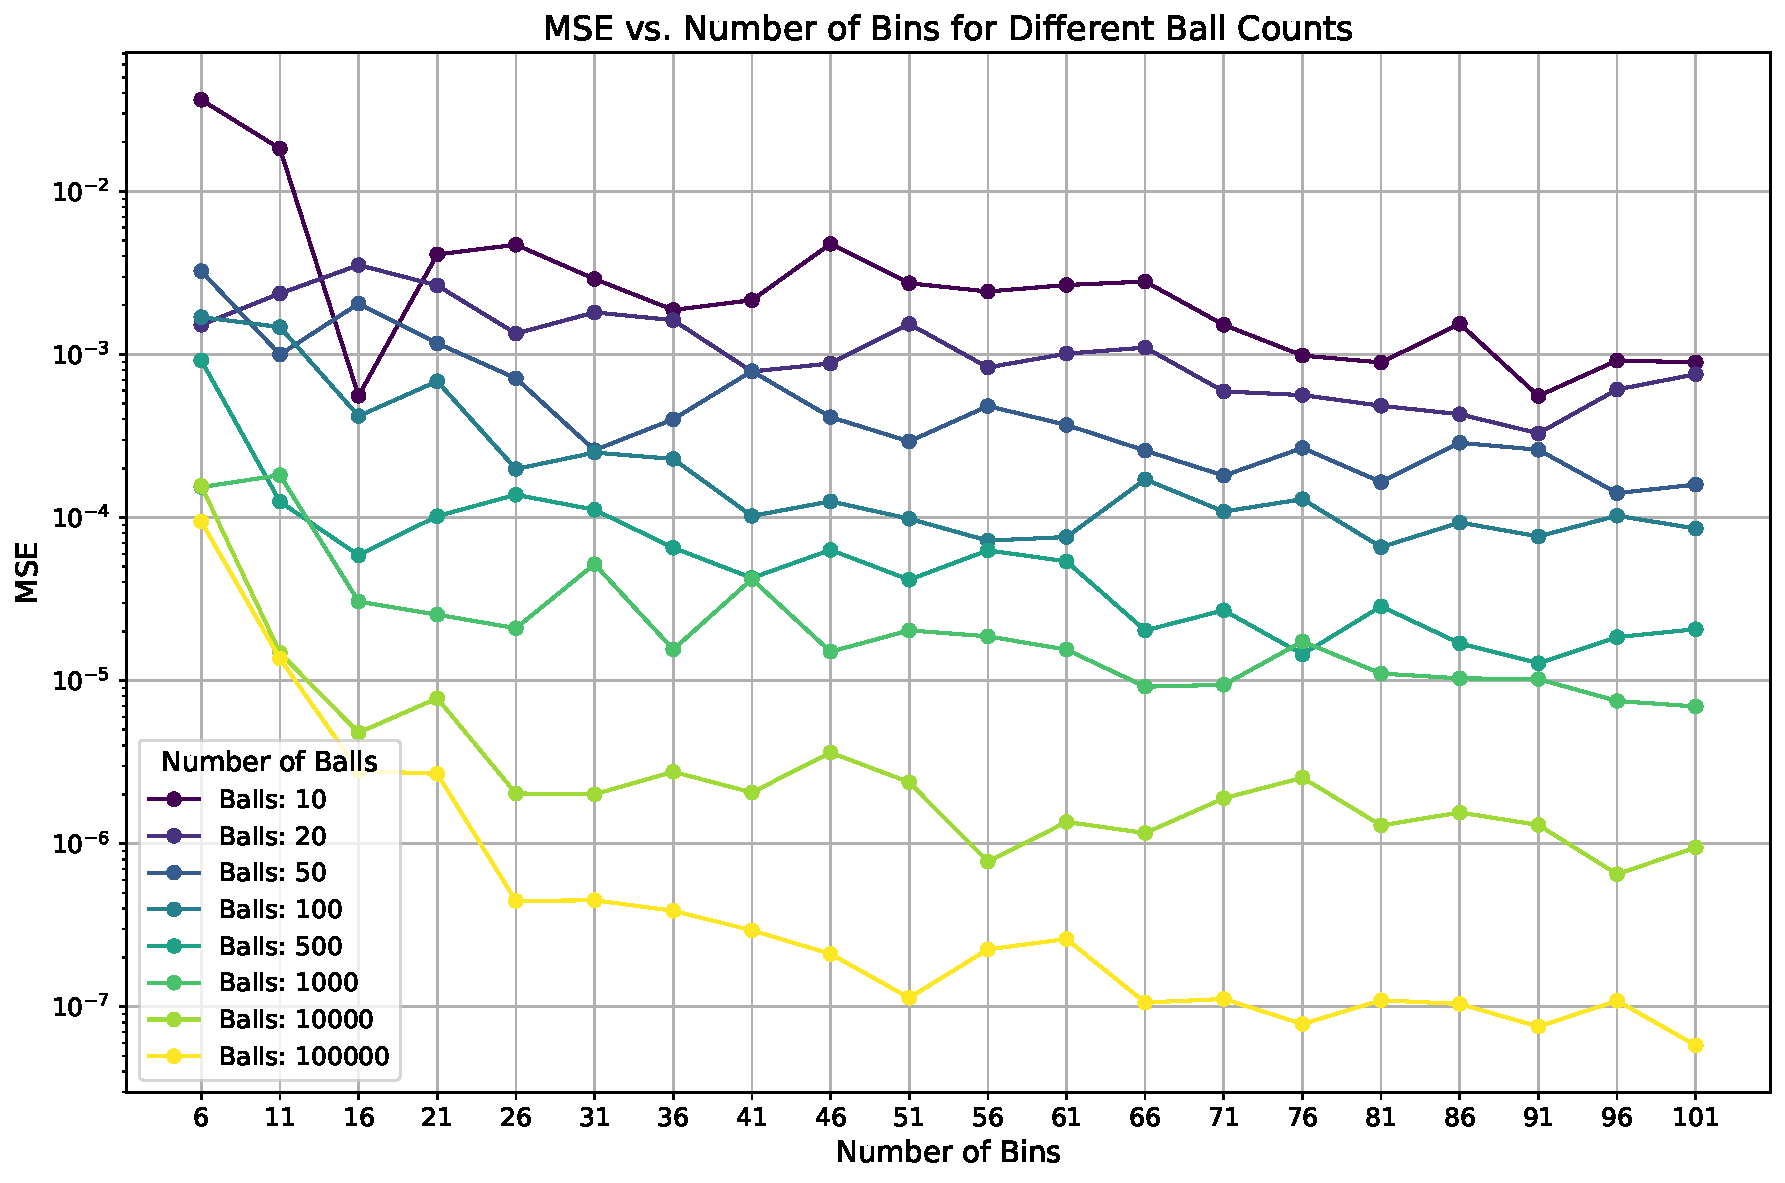
\includegraphics[width=1\linewidth]{plot.pdf}
    \caption{Mean square error analysis between the empirical results and the theoretical normal distribution across varying sample sizes and numbers of bins.}
    \label{fig:error_analysis}
\end{figure*}

\section{Usued Tools}
For the creation of the plots, TikZ+PGF has been used and, Figure~\ref{fig:error_analysis}, has been generating using a Python notebook that can be found in the project files with the name \texttt{data.ipynb}.

\printbibliography

\end{document}
